

\begin{minipage}{.67\linewidth}
Spillet krig (warGame) er et kortspil for to personer. Et almindeligt
spil kort med 52 kort blandes og deles mellem de to spillere. Hver
spiller holder sin bunke kort i hånden med billedsiden
nedaf. Spillerne spiller nu hver et kort ud på bordet fra toppen af
deres bunke. Spilleren der spiller det højeste kort vinder kortene på
bordet og disse kort placeres i bunden af vinderens bunke. I tilfælde
af at der spilles to ens kort (f.eks. to 7'ere) er der krig.
\end{minipage}\hfill
\begin{minipage}{.26\linewidth}
  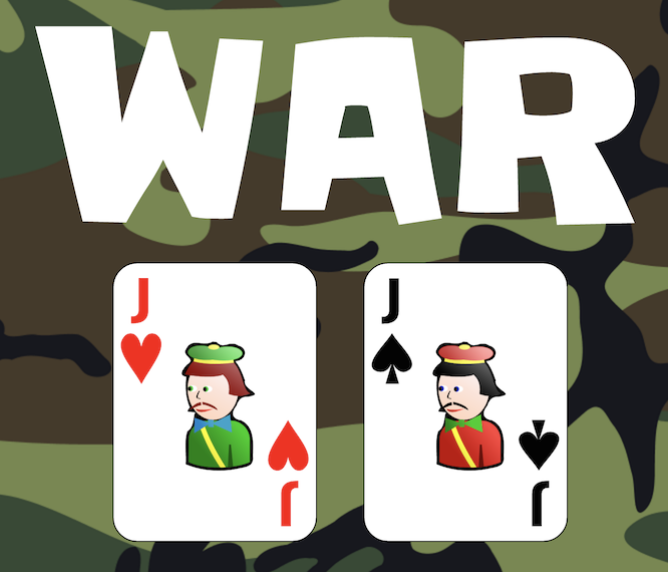
\includegraphics[width=.99\linewidth]{wargame.png}
\end{minipage}

Hver spiller spiller nu et ekstra kort ud på bordet fra toppen af
deres bunke men med billedsiden nedaf. Herefter fortsætter spillet
indtil en af spillerne vinder bunken på bordet. I tilfælde af at en
spiller løber tør for kort taber spilleren. I det specielle og meget
sjældne tilfælde at de to spillere samtidig løber tør for kort er der
tale om uafgjort.

I denne opgave skal der arbejdes mod at få computeren til at spille
kortspillet krig mod sig selv. Vi er i sidste ende interesseret i at
få viden om hvormange udspil en spiller i gennemsnit skal foretage før
et spil er afgjort samt hvor ofte spillet ender uafgjort.

Opgaven er delt i tre dele. I den første delopgave skal der arbejdes
mod at finde metoder til at blande og dele kort fra en bunke. I den
anden delopgave skal der arbejdes mod at få computeren til at spille
mod sig selv. Endelig skal der i den tredie delopgave arbejdes mod at
lave statistik på et antal kørsler af spillet.
